\subsection{sampling}	
\begin{frame}\frametitle{sampling and quantization}\framesubtitle{sampling}
		\vspace{-5mm}
        \begin{equation}\nonumber
			T_{\mathrm{S}} = \frac{1}{f_{\mathrm{S}}} 
		\end{equation}
		\begin{figure}
			\centering
				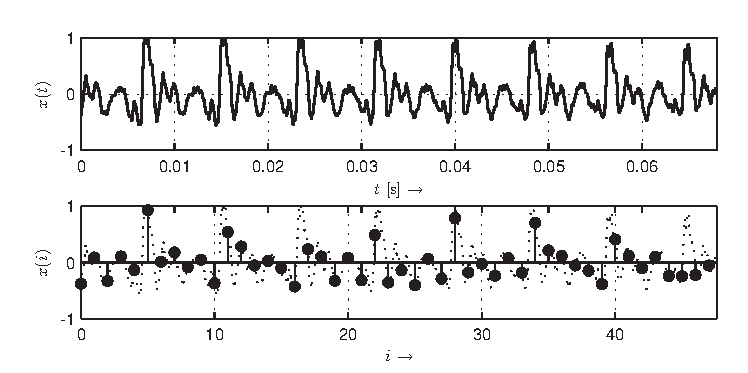
\includegraphics[scale=.6]{\AcaGraph/sampling}
			\label{fig:sampling}
		\end{figure}
		\pause
		typical sample rates
		\begin{itemize}
			\item	\unit[8-16]{kHz}: speech (phone)
			\item	\unit[44.1-48]{kHz}: (consumer) audio/music
			\item	higher: production audio
		\end{itemize}
	\end{frame}	

	\begin{frame}\frametitle{sampling and quantization}\framesubtitle{sampling ambiguity 1/4}
        \begin{center}
            \animategraphics[scale=.8,step]{1}{graph/samplingambi/samplingambi_}{1}{6}        
        \end{center}
		%\begin{figure}
			%\centering
				%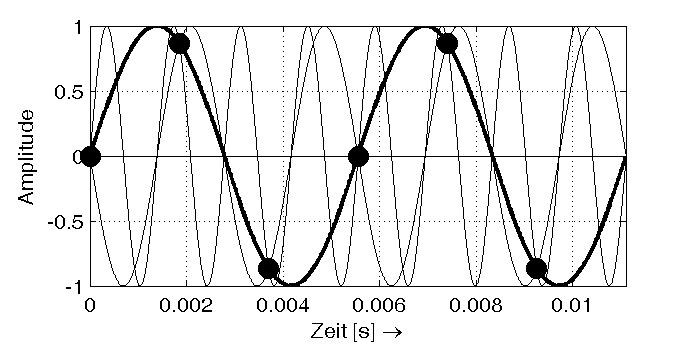
\includegraphics[scale=1.0]{Graph/sampling2}
		%\end{figure}
	\end{frame}
	
	\begin{frame}\frametitle{sampling and quantization}\framesubtitle{sampling ambiguity 2/4}
		\begin{eqnarray}
			f_0 &=& [\unit[1, 5, 7]{kHz}]\\
			f_{\mathrm{S}} &=& \unit[6]{kHz}
		\end{eqnarray}
		\begin{figure}
			\centering
				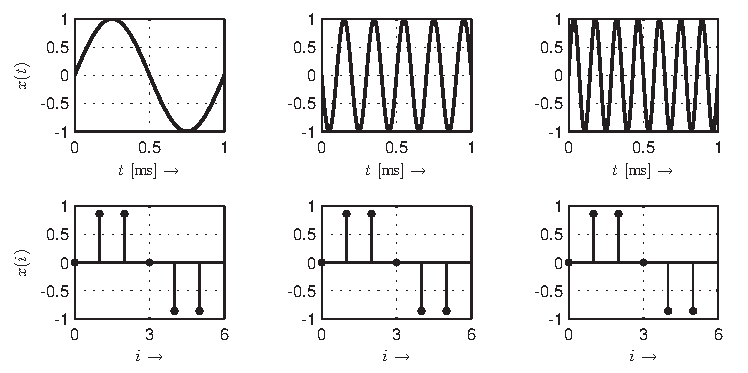
\includegraphics[scale=.7]{\AcaGraph/samplingambig}
				\label{fig:samplingambig}
		\end{figure}
	\end{frame}	
	
	\begin{frame}\frametitle{sampling and quantization}\framesubtitle{sampling ambiguity 3/4}
		\textbf{wagon wheel effect}
		\invisible<2->{
		\begin{figure}
			\begin{center}
				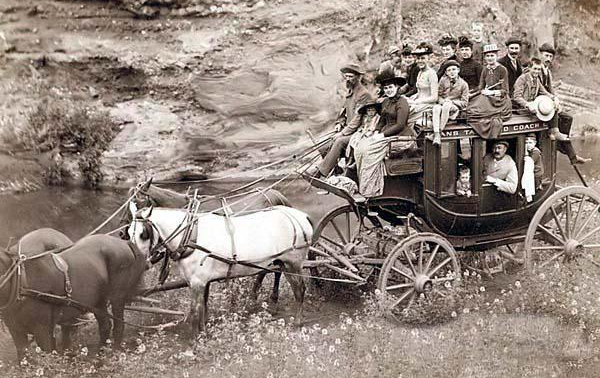
\includegraphics[scale=.4]{Graph/Stagecoach-Western}
			\end{center}
		\end{figure}
		}
		\visible<2->{
			\vspace{-60mm}
			\begin{figure}
				\begin{center}
					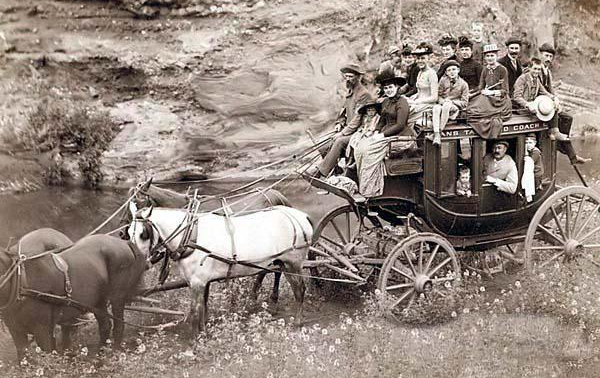
\includegraphics[scale=.2]{Graph/Stagecoach-Western}
				\end{center}
			\end{figure}
			\begin{enumerate}
				\item	$f_{wheel} < \frac{f_S}{2}$: speeding up
				\pause
				\item	$\frac{f_S}{2} < f_{wheel} < f_S$: slowing down
				\pause
				\item	$f_{wheel} = f_S$: standing still
				\pause
				\item	$\ldots$
			\end{enumerate}
		}
	\end{frame}

	\begin{frame}\frametitle{sampling and quantization}\framesubtitle{sampling ambiguity 4/4}
        \url{http://youtu.be/uENITui5_jU}
	\end{frame}	
	\begin{frame}\frametitle{sampling and quantization}\framesubtitle{sampling}
		\begin{itemize}
			\item[]	$x(t) \mapsto X(\jom)$
				\vspace{-6mm}
				\begin{figure}
					\flushright
						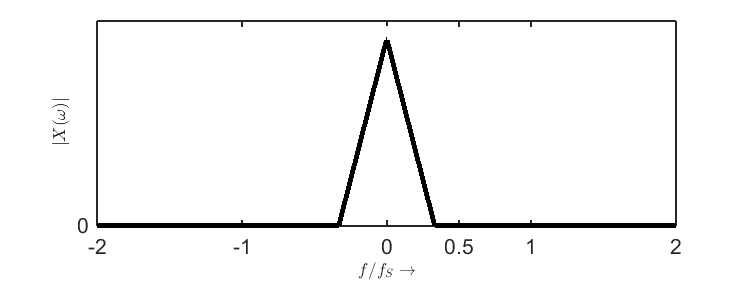
\includegraphics[scale=.4]{Graph/spectrum_sampling_1}
				\end{figure}
			
			\pause
			\item[]	$x(t)\cdot \delta_T \mapsto X(\jom)\ast \delta_{\omega_T}$
				\vspace{-6mm}
				\begin{figure}
					\flushright
						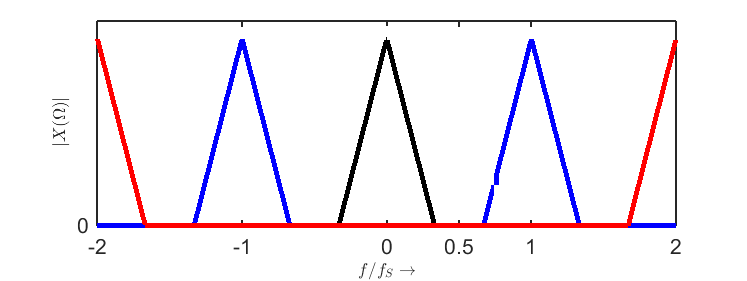
\includegraphics[scale=.4]{Graph/spectrum_sampling_2}
				\end{figure}
		\end{itemize}		
			\pause
        \begin{center}
            \animategraphics[scale=.5,autoplay,loop]{10}{graph/SpectralAliasing/aliasing_}{1}{101}        
        \end{center}
	\end{frame}
	
	\begin{frame}\frametitle{sampling and quantization}\framesubtitle{sampling theorem}
		\vspace{-10mm}
%		\only<1>{
        \begin{flushright}
			 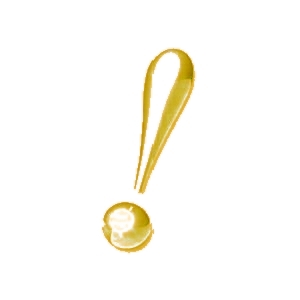
\includegraphics[scale=.25]{Graph/exclamation-mark}
		\end{flushright}
 %       }
		\begin{block}{sampling theorem}
			\centering
			A sampled audio signal can  be reconstructed \textbf{without loss of information} if the sample rate $f_{\mathrm{S}}$ is higher than twice the bandwidth $f_{\mathrm{max}}$  of the signal.
			\begin{equation}\label{eq:sample_theorem}	
				f_{\mathrm{S}} > 2\cdot f_{\mathrm{max}}
			\end{equation}
		\end{block}
        %\begin{quote}
             %``The intuitive justification is that, if x(t) contains no frequencies higher than \nicefrac{f_\mathrm{max}, it cannot change to a substantially new value in a time less than one-half cycle of the highest frequency".
        %\end{quote}
	\end{frame}
	
	\begin{frame}\frametitle{sampling and quantization}\framesubtitle{sampling: aliasing}
		\begin{figure}
			\begin{center}
				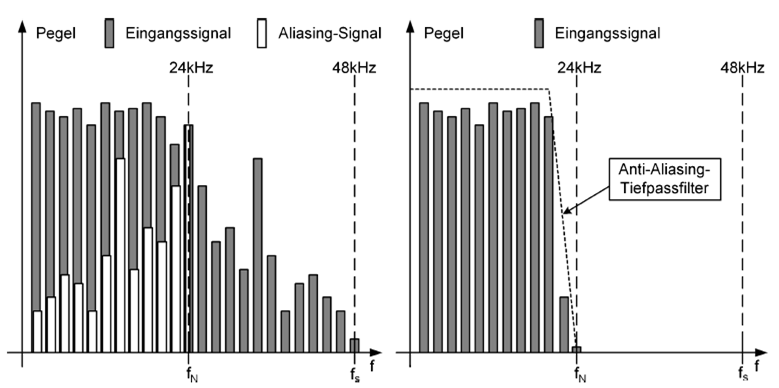
\includegraphics[scale=0.5]{Graph/aliasing}
			\end{center}
		\end{figure} 
	\end{frame}	

	\begin{frame}\frametitle{sampling and quantization}\framesubtitle{sampling: aliasing examples 1/2}
        \vspace{-5mm}
        audio example: sinesweep 100--10k at 24, 12, 6k
        \begin{columns}
            \column{.7\textwidth}
            \vspace{-5mm}
            \begin{figure}
                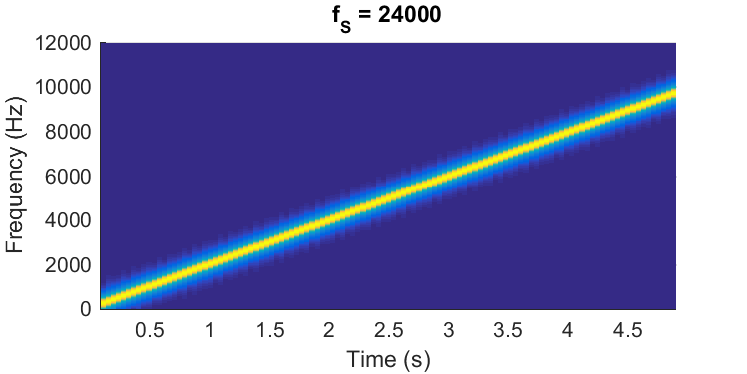
\includegraphics[scale=.35]{graph/sinealiasing_1}
            \end{figure}
            \visible<2->{
            \vspace{-6mm}
            \begin{figure}
                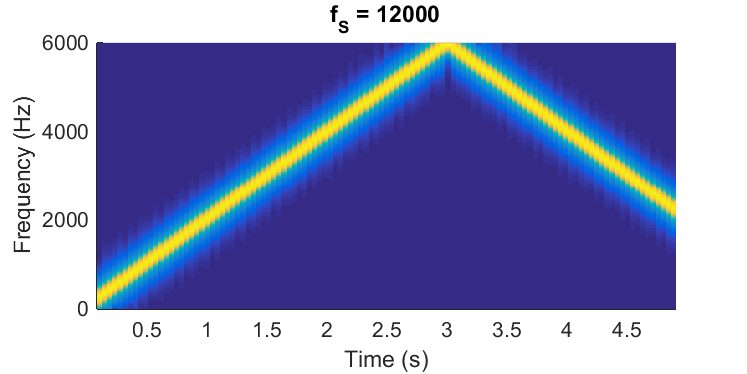
\includegraphics[scale=.35]{graph/sinealiasing_2}
            \end{figure}
            }
            \visible<3->{
            \vspace{-6mm}
            \begin{figure}
                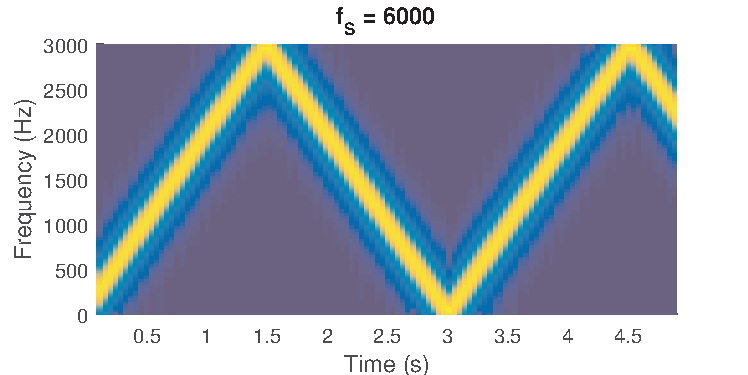
\includegraphics[scale=.35]{graph/sinealiasing_3}
            \end{figure}
            }
            \column{.3\textwidth}
            
            \includeaudio{audio/sinealiasing_1.mp3}
            %\begin{figure}
                %
\includegraphics[scale=.05]{graph/SpeakerIcon}
            %\end{figure}
            %\vspace{-3mm}
            %sinealiasing\_1.wav
            \bigskip
            \bigskip
            \bigskip
            \bigskip
            \bigskip
            
            \visible<2->{
            \includeaudio{audio/sinealiasing_2.mp3}
            %\begin{figure}
                %
\includegraphics[scale=.05]{graph/SpeakerIcon}
            %\end{figure}
            %\vspace{-3mm}
            %sinealiasing\_2.wav
            \bigskip
            \bigskip
            \bigskip
            \bigskip
            \bigskip
           }
            
            \visible<3->{
            \includeaudio{audio/sinealiasing_3.mp3}
            %\begin{figure}
                %
\includegraphics[scale=.05]{graph/SpeakerIcon}
            %\end{figure}
            %\vspace{-3mm}
            %sinealiasing\_3.wav
            }
        \end{columns}
		%\begin{itemize}
			%\item	original (\unit[44.1]{kHz})
					%\begin{figure}
						%\includemovie[poster=graph/SpeakerIcon.png,mouse=true]{1cm}{1cm}{audio/bigband.wav}
					%\end{figure}
			%\item	downsampled (\unit[11.025]{kHz}) \textit{without} aliasing filter
					%\begin{figure}
						%\includemovie[poster=graph/SpeakerIcon.png,mouse=true]{1cm}{1cm}{audio/bigbandds.wav}
					%\end{figure}
			%\item	downsampled (\unit[11.025]{kHz}) \textit{with} aliasing filter
					%\begin{figure}
						%\includemovie[poster=graph/SpeakerIcon.png,mouse=true]{1cm}{1cm}{audio/bigbandds_proper.wav}
					%\end{figure}
		%\end{itemize}
	\end{frame}	

	\begin{frame}\frametitle{sampling and quantization}\framesubtitle{sampling: aliasing examples 2/2}
    \begin{itemize}
        \item \textbf{bigband}
        \begin{itemize}
            \item   original (\unit[48]{kHz}): \includeaudio{audio/bigband.mp3}
            \item   samples discarded (\unit[6]{kHz}): \includeaudio{audio/bigbandds8.mp3}
            \item   downsampling  w/ anti-aliasing filter (\unit[6]{kHz}): \includeaudio{audio/bigbandds8_proper.mp3}
        \end{itemize}
        \pause
        \bigskip
        \item   \textbf{sax}
        \begin{itemize}
            \item   original (\unit[48]{kHz}): \includeaudio{audio/alto-sax.mp3}
            \item   samples discarded (\unit[6]{kHz}): \includeaudio{audio/alto-saxds8.mp3}
            \item   downsampling w/ anti-aliasing filter (\unit[6]{kHz}): \includeaudio{audio/alto-saxds8_proper.mp3}
        \end{itemize}
    \end{itemize}
	\end{frame}
	
	\begin{frame}\frametitle{sampling and quantization}\framesubtitle{sampling: signal pre \& post processing}
        \begin{enumerate}
            \item[]   continuous input signal
            \pause
            \item   \textbf{anti-aliasing filter}
            \pause
            \item[] filtered continuous input signal
            \pause
            \item   \textbf{sampling}
            \pause
            \item[] sampled input signal
            \pause
            \item   \textbf{reconstruction filter}
            \pause
            \item[] continuous output signal
        \end{enumerate}
	\end{frame}
